\documentclass[tikz]{standalone}
\usepackage{pgfplots}
\pgfplotsset{compat=1.15}
\usepackage{mathrsfs}
\usetikzlibrary{arrows,calc}
\usepackage{tkz-euclide}
\usepackage{fp}
\pagestyle{empty}

\definecolor{AngleClr}{rgb}{0,0.39215686274509803,0}
\definecolor{ShapeClr}{rgb}{0.6,0.2,0}
\definecolor{BlueClr}{RGB}{5,81,163}

\begin{document}

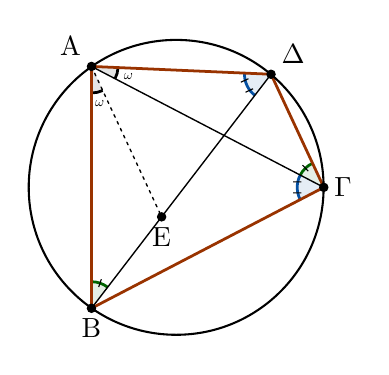
\begin{tikzpicture}[scale=.75]
\tkzSetUpLine[line width=1pt,color=black]
\tkzSetUpPoint[fill=black]

\tkzDefPoint(125:2.5){A}
\tkzDefPoint(235:2.5){B}
\tkzDefPoint(0:2.5){C}
\tkzDefPoint(50:2.5){D}

\tkzFindAngle(D,A,C) \tkzGetAngle{angleDAC}
\FPeval{\result}{90 - \angleDAC}
\tkzDefShiftPoint[A](\result:4){EE}


\tkzInterLL(A,EE)(B,D) \tkzGetPoint{E}

\tkzDefTriangleCenter[circum](A,B,C) \tkzGetPoint{O}

\tkzFillPolygon[fill=white](A,B,C,D)

\tkzFillAngles[fill=AngleClr,size=.45,fill opacity=0.1](D,B,A D,C,A)
\tkzMarkAngles[mark=|,mksize=1.5,line width=1pt,size=.45,color=AngleClr](D,B,A D,C,A)

\tkzFillAngles[fill=BlueClr,size=.45,fill opacity=0.1](A,D,B A,C,B)
\tkzMarkAngles[mark=||,mksize=1.5,line width=1pt,size=.45,color=BlueClr](A,D,B A,C,B)

\tkzFillAngles[fill=black,size=.45,fill opacity=0.1](B,A,E C,A,D)
\tkzMarkAngles[line width=1pt,size=.45,color=black](B,A,E C,A,D)
\tkzLabelAngles[pos=1.3,scale=0.5](B,A,E C,A,D){$\omega$}

\tkzDrawSegments[line width=0.5pt,color=black](A,C B,D)

\tkzDrawSegments[line width=0.5pt,color=black,dashed,dash pattern=on 1pt off 1.75pt](A,E)

\tkzDrawPolygon[color=ShapeClr](A,B,C,D)
\tkzDrawCircle[line width=0.75pt,color=black](O,A)

\tkzDrawPoints[size=3](A,B,C,D,E)

\tkzLabelPoint[above left](A){$\rm A$}
\tkzLabelPoint[below](B){$\rm B$}
\tkzLabelPoint[right](C){$\rm \Gamma$}
\tkzLabelPoint[above right](D){$\rm \Delta$}
\tkzLabelPoint[below](E){$\rm E$}


% \tkzLabelSegments[scale=0.75,above,sloped,pos=0.4](A,C){$\rm \mu$}
% \tkzLabelSegments[scale=0.75,above,sloped](B,D){$\rm \lambda$}

\end{tikzpicture}
\end{document}
